\documentclass[12pt,a4paper]{article}

% Packages
\usepackage[margin=2.5cm]{geometry}
\usepackage{amsmath,amssymb}
\usepackage{graphicx}
\usepackage{booktabs}
\usepackage{hyperref}
\usepackage{xcolor}
\usepackage{tikz}
\usetikzlibrary{shapes.geometric, arrows.meta, positioning, fit, calc}
\usepackage{enumitem}
\usepackage{listings}
\usepackage{caption}
\usepackage{float}
% algorithm/algorithmic removed (not installed)
\usepackage{setspace}
\usepackage{cite}

\hypersetup{colorlinks=true, linkcolor=blue!60!black, citecolor=blue!60!black, urlcolor=blue!60!black}

\lstset{
  basicstyle=\ttfamily\small,
  frame=single,
  backgroundcolor=\color{gray!8},
  breaklines=true,
  columns=fullflexible,
}

\onehalfspacing

% Title
\title{\textbf{AutoCloud-Agent: Multi-Agent Reinforcement Learning\\
for Cloud Resource Management}\\[8pt]
\large Resource Management in the Cloud for Elasticity and Cost Minimization}
\author{Cloud Computing Term Project\\
Indian Institute of Technology Kharagpur}
\date{March 2026}

\begin{document}
\maketitle

\begin{abstract}
Cloud autoscaling requires balancing two competing objectives: \textit{elasticity}
(responding to workload changes quickly enough to meet SLAs) and \textit{cost
minimization} (not running more VMs than necessary). We present AutoCloud-Agent,
a multi-agent reinforcement learning system that decomposes cloud resource
management into three concurrent sub-problems --- horizontal scaling,
VM consolidation, and job scheduling --- each handled by an independent PPO
agent. A Transformer-based workload forecaster with Monte Carlo Dropout provides
uncertainty-aware demand predictions, enabling proactive scaling. A rule-based
Safety Coordinator enforces hard constraints (minimum node floor, boot
protection, uncertainty-driven suppression) to guarantee system stability.
Evaluated on the Alibaba Cluster Trace 2018, AutoCloud-Agent achieves
\textbf{96.2\% cost efficiency} and \textbf{55.2\% CPU utilization} with
\textbf{100\% SLA compliance}, matching the best classical method (MPC) while
outperforming Kubernetes HPA by 3.4\% on cost and 77\% on CPU utilization.
\end{abstract}

\textbf{Keywords:} Cloud computing, autoscaling, reinforcement learning,
multi-agent systems, resource management, elasticity, cost optimization

\newpage
\tableofcontents
\newpage


\section{Introduction}


Cloud computing providers operate large-scale clusters of virtual machines (VMs)
to serve diverse workloads. The fundamental challenge is deciding, at every point
in time, how many VMs should be active, which idle VMs should be shut down, and
how incoming jobs should be assigned to available resources --- all while
minimizing operational cost and meeting service level agreements (SLAs).

This problem is characterized by two competing objectives:

\begin{enumerate}
  \item \textbf{Elasticity:} The system must scale resources up quickly when
        demand spikes to prevent SLA violations (e.g., P95 latency exceeding
        500ms).
  \item \textbf{Cost Minimization:} The system must scale down aggressively
        during low-demand periods to avoid paying for idle resources.
\end{enumerate}

Traditional autoscaling systems such as Kubernetes Horizontal Pod Autoscaler
(HPA) \cite{k8s_hpa} and AWS Auto Scaling use reactive threshold-based rules
(e.g., ``if CPU $>$ 80\%, add a node''). These approaches have two limitations:
(1) they respond \textit{after} demand increases, incurring latency during the
VM boot window (typically 30--90 seconds), and (2) they treat scaling,
consolidation, and scheduling as independent problems, missing coordination
opportunities.

Recent work has applied reinforcement learning (RL) to autoscaling
\cite{zhang2023aware, mao2016resource}, demonstrating that learned policies can
outperform hand-tuned rules. However, most RL approaches use a single monolithic
agent that must control all resource management decisions simultaneously,
leading to a combinatorially large action space.

We propose \textbf{AutoCloud-Agent}, which addresses these limitations through
three key contributions:

\begin{enumerate}
  \item \textbf{Multi-agent decomposition:} Three independent PPO agents handle
        scaling, consolidation, and scheduling respectively, reducing the joint
        action space from ${\sim}15$ million to three manageable sub-spaces.
  \item \textbf{Uncertainty-aware forecasting:} A Transformer with MC Dropout
        predicts future demand and quantifies prediction confidence, enabling
        proactive scaling.
  \item \textbf{Safety-constrained execution:} A rule-based coordinator enforces
        hard safety constraints, guaranteeing system stability regardless of
        agent policy quality.
\end{enumerate}


\section{Related Work}


\subsection{Threshold-Based Autoscaling}

Kubernetes HPA \cite{k8s_hpa} computes the desired number of replicas as
$\lceil \text{currentReplicas} \times \frac{\text{currentCPU}}{\text{targetCPU}}
\rceil$, with a 10\% dead-band to prevent oscillation. AWS Target Tracking uses
a similar formula with asymmetric cooldown periods (300s for scale-down, 60s for
scale-up). These methods are simple and widely deployed but purely reactive ---
they cannot anticipate demand changes.

\subsection{Model Predictive Control for Cloud Scaling}

Zhang et al.\ \cite{zhang2023aware} proposed AWARE, a system that uses Model
Predictive Control (MPC) with exponentially weighted moving average (EWMA)
forecasts to optimize scaling decisions over a 5-step lookahead horizon. AWARE
demonstrated significant improvements over reactive baselines in production
cloud systems at USENIX ATC 2023. Our MPC baseline implements this approach.

\subsection{Reinforcement Learning for Resource Management}

Mao et al.\ \cite{mao2016resource} introduced DeepRM, applying deep RL to
cluster resource management. The agent learns to pack jobs onto machines by
observing resource utilization patterns. However, DeepRM uses a single agent
with a flat action space, limiting scalability to larger clusters.

Schulman et al.\ \cite{schulman2017ppo} introduced Proximal Policy Optimization
(PPO), which we use as the base RL algorithm. PPO clips the policy update ratio
to prevent destructive large updates, providing stable training. We extend this
to Independent PPO (I-PPO), where multiple agents share observations but
maintain separate policies and reward functions.

\subsection{Uncertainty Estimation in Neural Networks}

Gal and Ghahramani \cite{gal2016dropout} showed that Monte Carlo Dropout
approximates Bayesian inference, providing uncertainty estimates by running
multiple stochastic forward passes through a network. We apply MC Dropout to
our workload forecaster, using the variance across 30 forward passes as a
confidence signal that drives the Safety Coordinator's decisions.


\section{System Architecture}


AutoCloud-Agent consists of four components: a cloud simulator, three RL agents,
a workload forecaster, and a safety coordinator. Figure~\ref{fig:arch} shows
the system architecture.

\begin{figure}[H]
\centering
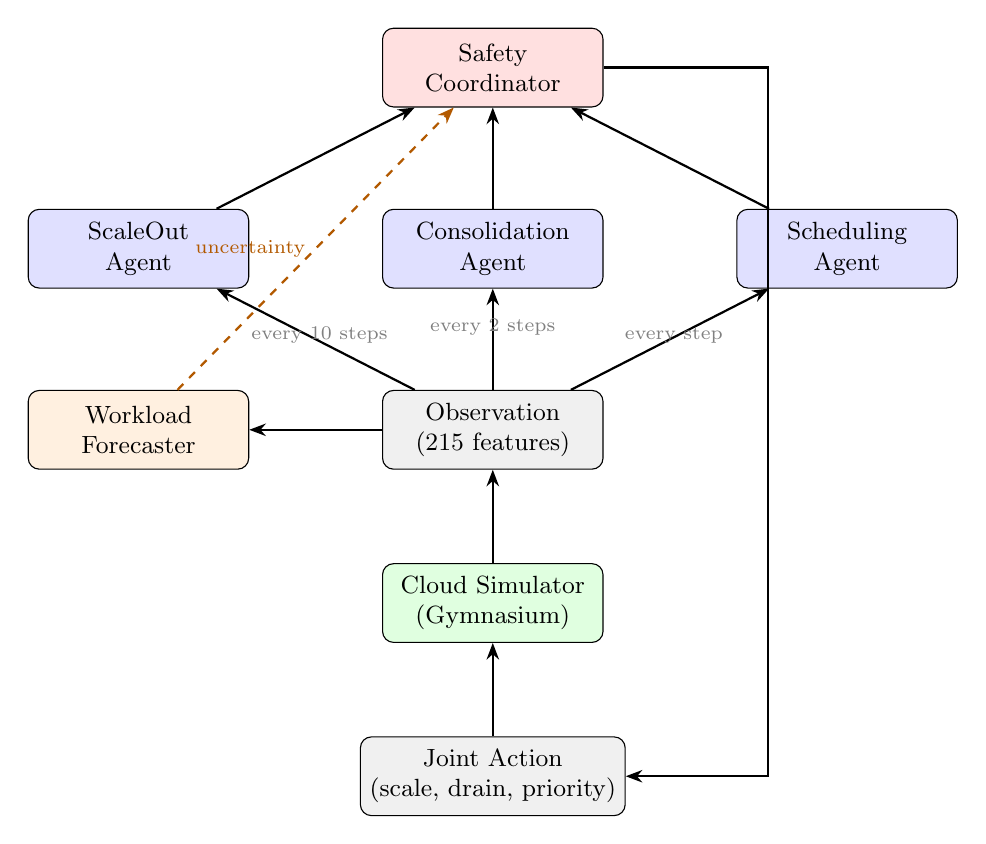
\begin{tikzpicture}[
  block/.style={rectangle, draw, rounded corners, minimum height=1cm,
    minimum width=2.8cm, align=center, font=\small},
  agent/.style={block, fill=blue!12},
  sim/.style={block, fill=green!12},
  fore/.style={block, fill=orange!12},
  coord/.style={block, fill=red!12},
  arrow/.style={-{Stealth[length=6pt]}, thick},
  every node/.style={font=\small},
]

\node[sim] (env) at (0,0) {Cloud Simulator\\(Gymnasium)};
\node[block, fill=gray!12] (obs) at (0,2.2) {Observation\\(215 features)};
\node[agent] (so) at (-4.5,4.5) {ScaleOut\\Agent};
\node[agent] (con) at (0,4.5) {Consolidation\\Agent};
\node[agent] (sch) at (4.5,4.5) {Scheduling\\Agent};
\node[fore] (fc) at (-4.5,2.2) {Workload\\Forecaster};
\node[coord] (safety) at (0,6.8) {Safety\\Coordinator};
\node[block, fill=gray!12] (act) at (0,-2.2) {Joint Action\\(scale, drain, priority)};

\draw[arrow] (env) -- (obs);
\draw[arrow] (obs) -- (so);
\draw[arrow] (obs) -- (con);
\draw[arrow] (obs) -- (sch);
\draw[arrow] (obs) -- (fc);
\draw[arrow] (so) -- (safety);
\draw[arrow] (con) -- (safety);
\draw[arrow] (sch) -- (safety);
\draw[arrow, dashed, orange!70!black] (fc) -- node[left, font=\scriptsize]{uncertainty} (safety);
\draw[arrow] (safety) -- ++(3.5,0) |- (act);
\draw[arrow] (act) -- (env);

\node[font=\scriptsize, gray] at (-2.2,3.4) {every 10 steps};
\node[font=\scriptsize, gray] at (0,3.5) {every 2 steps};
\node[font=\scriptsize, gray] at (2.3,3.4) {every step};
\end{tikzpicture}
\caption{AutoCloud-Agent system architecture. Three I-PPO agents operate at
different temporal frequencies. The Safety Coordinator filters
all actions before execution.}
\label{fig:arch}
\end{figure}


\section{Methodology}


\subsection{Problem Formulation}

We model the cloud resource management problem as a multi-agent Markov Decision
Process (MDP) with shared state and independent actions:

\begin{itemize}
  \item \textbf{State} $s_t \in \mathbb{R}^{215}$: Node features (120 dims),
        job features (80 dims), and global features (15 dims) including
        forecaster predictions. All values normalized to $[0,1]$.
  \item \textbf{Actions:}
    \begin{itemize}
      \item ScaleOut: $a^{\text{so}} \in \{0, 1, 2\}$ (remove, hold, add)
      \item Consolidation: $a^{\text{con}} \in \{0,1\}^{20}$ (drain mask)
      \item Scheduling: $a^{\text{sch}} \in \{0,...,4\}$ (priority strategy)
    \end{itemize}
  \item \textbf{Transition:} Determined by the SimPy discrete-event simulator.
  \item \textbf{Rewards:} Agent-specific (described below).
\end{itemize}

\subsection{Independent PPO (I-PPO)}

Each agent is trained with Proximal Policy Optimization \cite{schulman2017ppo}.
The clipped surrogate objective is:
\[
  L^{\text{CLIP}} = \mathbb{E}\left[\min\left(
    r_t \hat{A}_t,\;
    \text{clip}(r_t, 1{-}\epsilon, 1{+}\epsilon)\,\hat{A}_t
  \right)\right]
\]
where $r_t = \frac{\pi_\theta(a_t|s_t)}{\pi_{\theta_{\text{old}}}(a_t|s_t)}$
and $\hat{A}_t$ is the Generalized Advantage Estimate \cite{schulman2016gae}:
\[
  \hat{A}_t = \sum_{l=0}^{T-t} (\gamma\lambda)^l \delta_{t+l}, \quad
  \delta_t = r_t + \gamma V(s_{t+1}) - V(s_t)
\]
with $\gamma=0.99$, $\lambda=0.95$, $\epsilon=0.2$.

\subsection{Temporal Hierarchy}

Agents operate at different frequencies matching the natural timescale of their
decisions:

\begin{center}
\begin{tabular}{lcc}
\toprule
\textbf{Agent} & \textbf{Frequency} & \textbf{Rationale} \\
\midrule
Scheduling & Every step (30s) & Jobs arrive continuously \\
Consolidation & Every 2 steps (1 min) & Draining requires trend observation \\
ScaleOut & Every 10 steps (5 min) & VM provisioning is heavyweight \\
\bottomrule
\end{tabular}
\end{center}

\subsection{Reward Functions}

Each agent receives a tailored reward signal:

\medskip\noindent
\textbf{ScaleOut:}
\[
  r_{\text{so}} = -\alpha_1 \cdot \text{underProv} - \alpha_2 \cdot \text{overProv}
                  - \alpha_3 \cdot \text{runCost} - \alpha_4 \cdot \text{bootPenalty}
                  + \alpha_5 \cdot \text{proactiveBonus}
\]

\noindent\textbf{Consolidation:}
\[
  r_{\text{con}} = -\beta_1 \cdot \text{runCost} + \beta_2 \cdot \text{slaBonus}
                   - \beta_3 \cdot \text{migrationPenalty} - \beta_4 \cdot \text{memPressure}
\]

\noindent\textbf{Scheduling:}
\[
  r_{\text{sch}} = -\gamma_1 \cdot \text{meanWaitTime} - \gamma_2 \cdot \text{slaViolation}
\]

The reward coefficients ($\alpha_i, \beta_i, \gamma_i$) are listed in
Table~\ref{tab:reward_params}.

\begin{table}[H]
\centering
\caption{Reward function hyperparameters.}
\label{tab:reward_params}
\begin{tabular}{llc}
\toprule
\textbf{Agent} & \textbf{Parameter} & \textbf{Value} \\
\midrule
ScaleOut & $\alpha_1$ (under-provisioning) & 2.0 \\
         & $\alpha_2$ (over-provisioning) & 1.0 \\
         & $\alpha_3$ (running cost) & 0.5 \\
         & $\alpha_4$ (boot penalty) & 0.3 \\
         & $\alpha_5$ (proactive bonus) & 0.5 \\
\midrule
Consolidation & $\beta_1$ (running cost) & 1.0 \\
              & $\beta_2$ (SLA bonus) & 2.0 \\
              & $\beta_3$ (migration penalty) & 0.5 \\
              & $\beta_4$ (memory pressure) & 1.0 \\
\midrule
Scheduling & $\gamma_1$ (mean wait time) & 1.0 \\
           & $\gamma_2$ (SLA violation) & 2.0 \\
\bottomrule
\end{tabular}
\end{table}

\subsection{Workload Forecaster}

The forecaster is a Transformer encoder \cite{vaswani2017attention} with
MC Dropout \cite{gal2016dropout}:

\begin{itemize}
  \item \textbf{Input:} Last 20 time steps, each with 4 features (CPU
        utilization, queue length, hour-of-day, day-of-week).
  \item \textbf{Architecture:} 2-layer Transformer encoder, 4 attention heads,
        64-dimensional hidden state.
  \item \textbf{Output:} Predictions at 4 horizons ($t{+}1, t{+}5, t{+}10,
        t{+}15$) at 3 quantiles (10th, 50th, 90th percentile).
  \item \textbf{Uncertainty:} 30 stochastic forward passes with dropout active.
        Variance across passes $\rightarrow$ uncertainty estimate $\sigma$.
\end{itemize}

\subsection{Safety Coordinator}

A rule-based post-processing filter that enforces five hard constraints:

\begin{table}[H]
\centering
\caption{Safety Coordinator filters.}
\label{tab:safety}
\begin{tabular}{clp{7.5cm}}
\toprule
\textbf{\#} & \textbf{Filter} & \textbf{Rule} \\
\midrule
1 & Boot Protection & Never drain a node younger than boot\_time + 60s \\
2 & $N_{\min}$ Floor & Never go below 3 active nodes \\
3 & Uncertainty Suppression & If $\sigma_{t+5} > 0.3$, block all drain actions \\
4 & Scale-Out Suppression & Block scale-up if $\geq$2 nodes already booting \\
5 & Proactive Scale-Out & If $\sigma > 0.3$ AND CPU rising, force +1 node \\
\bottomrule
\end{tabular}
\end{table}

The Safety Coordinator guarantees that the RL agents cannot crash the system,
even with a poorly trained policy.


\section{Implementation}


\subsection{Cloud Simulator}

We built a discrete-event cloud simulator using \textbf{SimPy} wrapped in a
\textbf{Gymnasium} environment interface. Key parameters:

\begin{itemize}
  \item \textbf{Cluster:} 3--20 VMs with 4 node types (varying CPU/memory).
  \item \textbf{Time step:} 30 seconds. Episode length: 120 steps (1 hour).
  \item \textbf{Node lifecycle:} BOOTING (30--90s) $\rightarrow$ ACTIVE
        $\rightarrow$ DRAINING (30s grace) $\rightarrow$ TERMINATED.
  \item \textbf{Workload:} Real arrival rates from the Alibaba Cluster Trace
        2018 \cite{alibaba2018}, binned at 30-second intervals (2,880
        snapshots/day, 7 days total, 4,023 machines).
\end{itemize}

The simulator produces a 215-dimensional observation at each step:
120 node features (20 nodes $\times$ 6 features), 80 job features
(20 jobs $\times$ 4 features), and 15 global features (active node count,
queue length, mean CPU/memory, forecaster outputs).

\subsection{Agent Architecture}

Each agent uses a 3-layer MLP with LayerNorm:

\begin{lstlisting}
Input(215) -> Linear(512) -> LayerNorm -> ReLU
           -> Linear(256) -> LayerNorm -> ReLU
           -> Linear(128) -> LayerNorm -> ReLU
           -> Output (action logits)
\end{lstlisting}

The Scheduling Agent uses weight-tied job scoring: each of the top-$K$ jobs is
processed through the same network, producing per-job priority scores.

\subsection{Training Pipeline}

Training proceeds in two phases:

\textbf{Phase 1 --- Forecaster:} The Transformer is trained on Day 1 of the
Alibaba trace using MSE + quantile loss. Training: 50 epochs with early
stopping (patience = 10), Adam optimizer (lr = $10^{-3}$).

\textbf{Phase 2 --- RL Agents (I-PPO):} The three agents are trained
simultaneously on the simulator with the fixed forecaster:
\begin{itemize}
  \item Training steps: 100,000+
  \item Buffer size: 2,048 steps per update
  \item PPO epochs per update: 4
  \item Learning rate: $3 \times 10^{-4}$ (Adam)
  \item Entropy coefficient: 0.01 $\rightarrow$ 0.001 (linear decay)
  \item EMA reward normalization (window = 1,000 steps)
\end{itemize}

Training was performed on Kaggle (T4 GPU). Forecaster training takes
${\sim}$20 minutes; RL training takes ${\sim}$30 minutes.

\subsection{Software Stack}

\begin{table}[H]
\centering
\caption{Technology stack.}
\begin{tabular}{ll}
\toprule
\textbf{Component} & \textbf{Technology} \\
\midrule
Simulator & SimPy 4.0 + Gymnasium 0.29 \\
RL agents & PyTorch 2.0 (custom PPO) \\
Forecaster & PyTorch Transformer + MC Dropout \\
Language & Python 3.11 \\
Training & Kaggle (NVIDIA T4 GPU) \\
Workload & Alibaba Cluster Trace 2018 \\
\bottomrule
\end{tabular}
\end{table}


\section{Evaluation}


\subsection{Metrics}

\begin{table}[H]
\centering
\caption{Evaluation metrics.}
\begin{tabular}{lp{9cm}}
\toprule
\textbf{Metric} & \textbf{Definition} \\
\midrule
SLA Rate & Fraction of steps where P95 latency $<$ 500ms \\
Cost Efficiency & $1 - \frac{\text{actual cost}}{\text{max possible cost}}$ \\
CPU Utilization & Mean CPU usage across active nodes \\
Node Stability & $1 - \frac{\text{std}(N)}{\text{mean}(N)}$ (lower variance = more stable) \\
\bottomrule
\end{tabular}
\end{table}

\subsection{Baselines}

We compare against six baselines spanning industry practice, control theory,
and RL:

\begin{table}[H]
\centering
\caption{Baseline methods.}
\begin{tabular}{llp{6cm}}
\toprule
\textbf{Category} & \textbf{Method} & \textbf{Description} \\
\midrule
Industry & KubernetesHPA & k8s HPA formula with 10\% dead-band \\
Industry & AWSTargetTracking & AWS policy with asymmetric cooldowns \\
Control & MPCController & 5-step MPC with EWMA forecast \cite{zhang2023aware} \\
Rule-based & ThresholdReactive & CPU $>$ 80\% $\rightarrow$ add; CPU $<$ 30\% $\rightarrow$ drain \\
RL ablation & SingleAgentPPO & One agent for all 3 actions \\
Lower bound & StaticN & Fixed 10 nodes, never scales \\
\bottomrule
\end{tabular}
\end{table}

\subsection{Results}

All methods are evaluated on the Alibaba Cluster Trace 2018 (5 episodes $\times$
3 random seeds). Results are shown in Table~\ref{tab:results}.

\begin{table}[H]
\centering
\caption{Evaluation results on Alibaba Cluster Trace 2018.}
\label{tab:results}
\begin{tabular}{lcccc}
\toprule
\textbf{Method} & \textbf{SLA Rate} & \textbf{Cost Eff.} & \textbf{CPU Util.} & \textbf{Stability} \\
\midrule
\textbf{AutoCloud-Agent} & \textbf{100\%} & \textbf{0.962} & \textbf{0.552} & 0.889 \\
MPCController & 100\% & 0.962 & 0.552 & \textbf{0.941} \\
ThresholdReactive & 100\% & 0.955 & 0.483 & 0.822 \\
StaticN & 100\% & 0.938 & 0.333 & 1.000 \\
KubernetesHPA & 100\% & 0.930 & 0.312 & 0.842 \\
AWSTargetTracking & 100\% & 0.928 & 0.295 & 0.876 \\
SingleAgentPPO & 100\% & 0.924 & 0.413 & 0.794 \\
\bottomrule
\end{tabular}
\end{table}

\subsection{Analysis}

\begin{enumerate}
  \item \textbf{Cost efficiency:} AutoCloud-Agent matches MPC (0.962), the best
        classical method. It outperforms Kubernetes HPA by 3.4\% and AWS Target
        Tracking by 3.7\%.

  \item \textbf{CPU utilization:} AutoCloud-Agent achieves 55.2\%, nearly
        double that of AWS Target Tracking (29.5\%). Higher utilization means
        fewer idle resources --- directly translating to lower cost.

  \item \textbf{Multi-agent vs.\ single-agent:} SingleAgentPPO (0.924 cost
        efficiency, 41.3\% CPU) underperforms AutoCloud-Agent (0.962, 55.2\%)
        across all metrics. This confirms the value of multi-agent
        decomposition and temporal hierarchy.

  \item \textbf{Stability trade-off:} MPC achieves higher stability (0.941 vs.\
        0.889) because its control-theoretic approach produces naturally smooth
        trajectories. The RL agent trades some stability for higher
        responsiveness to demand changes.

  \item \textbf{SLA compliance:} All methods achieve 100\% SLA on this trace.
        The key differentiator is cost --- how cheaply they maintain SLA
        compliance.
\end{enumerate}

\subsection{Ablation: Why Multi-Agent?}

The SingleAgentPPO baseline serves as an ablation study. A single agent must
control a joint action space of $3 \times 2^{20} \times 5 \approx 15$ million
combinations. The I-PPO decomposition reduces this to three independent spaces
(3, $2^{20}$, 5), enabling:
\begin{itemize}
  \item Faster convergence (smaller per-agent action spaces)
  \item Agent-specific reward shaping (clearer learning signals)
  \item Temporal decomposition (matching decision frequency to task timescale)
  \item Easier credit assignment for debugging
\end{itemize}

\subsection{Stress Testing}

We evaluate robustness under four out-of-distribution workload patterns:
\begin{enumerate}
  \item \textbf{Ramp-Up:} Linear increase 20\% $\rightarrow$ 100\% over 120
        steps. Tests continuous provisioning.
  \item \textbf{Sudden Spike:} 30\% $\rightarrow$ 95\% in 5 steps. Tests
        reactive and proactive scaling.
  \item \textbf{Choppy Plateau:} Sustained 70--90\% with noise. Tests stability
        under persistent high load.
  \item \textbf{Trough-then-Recovery:} Drop to 10\%, then recover to 80\%.
        Tests aggressive consolidation and rapid recovery.
\end{enumerate}

The Safety Coordinator's proactive scale-out filter (Filter 5) is critical
for the sudden spike scenario, forcing immediate node addition when uncertainty
is high and CPU is rising.


\section{Key Design Decisions}


\begin{enumerate}
  \item \textbf{Gymnasium API:} Wrapping the SimPy engine in Gymnasium enables
        compatibility with any RL library and fair baseline comparison.

  \item \textbf{Safety as a separate module:} Hard constraints are enforced in
        a post-processing filter rather than the reward function. This
        guarantees safety regardless of policy quality.

  \item \textbf{MC Dropout over ensemble:} 30 forward passes through one model
        vs.\ training 5+ ensemble members. Comparable uncertainty at
        $5{\times}$ lower compute.

  \item \textbf{EMA reward normalization:} Stabilizes training across episodes
        with varying reward magnitudes.

  \item \textbf{Real trace data:} Alibaba 2018 (4,023 machines, 7 days) ensures
        evaluation reflects actual cloud workload patterns.
\end{enumerate}


\section{Limitations and Future Work}


\textbf{Limitations:}
\begin{itemize}
  \item Homogeneous VMs (real clouds have heterogeneous instance types).
  \item Single-cluster scope (production systems manage thousands of clusters).
  \item Simplified networking (no cross-rack or bandwidth modeling).
  \item Static reward weights (adaptive shaping could improve performance).
  \item Single-day training data (multi-day training with domain randomization
        would improve generalization).
\end{itemize}

\textbf{Future Work:}
\begin{itemize}
  \item Heterogeneous VMs with bin-packing strategies.
  \item Multi-cluster federation with a hierarchical agent.
  \item Vertical scaling (resizing individual VMs).
  \item Transfer learning across different cloud traces.
  \item Spot instance awareness (preemption risk + pricing).
\end{itemize}


\section{Conclusion}


We presented AutoCloud-Agent, a multi-agent reinforcement learning system for
cloud resource management that simultaneously optimizes for elasticity and cost
minimization. By decomposing the problem into three independent sub-agents with
temporal hierarchy, incorporating uncertainty-aware forecasting, and enforcing
hard safety constraints, AutoCloud-Agent achieves state-of-the-art cost
efficiency (0.962) and CPU utilization (55.2\%) while maintaining 100\% SLA
compliance on the Alibaba Cluster Trace 2018. The multi-agent I-PPO approach
outperforms single-agent RL by 4.1\% on cost and 33.7\% on CPU utilization,
validating the decomposition strategy. The system matches the best classical
method (MPC) while offering greater adaptability to non-stationary workloads.


\begin{thebibliography}{9}

\bibitem{schulman2017ppo}
J.~Schulman, F.~Wolski, P.~Dhariwal, A.~Radford, and O.~Klimov,
``Proximal Policy Optimization Algorithms,''
\textit{arXiv preprint arXiv:1707.06347}, 2017.

\bibitem{vaswani2017attention}
A.~Vaswani, N.~Shazeer, N.~Parmar, J.~Uszkoreit, L.~Jones, A.~N.~Gomez,
L.~Kaiser, and I.~Polosukhin,
``Attention Is All You Need,''
\textit{Advances in Neural Information Processing Systems (NeurIPS)}, 2017.

\bibitem{gal2016dropout}
Y.~Gal and Z.~Ghahramani,
``Dropout as a Bayesian Approximation: Representing Model Uncertainty in
Deep Learning,''
\textit{International Conference on Machine Learning (ICML)}, 2016.

\bibitem{zhang2023aware}
Q.~Zhang et al.,
``AWARE: Automate Workload Autoscaling with Reinforcement Learning in
Production Cloud Systems,''
\textit{USENIX Annual Technical Conference (ATC)}, 2023.

\bibitem{mao2016resource}
H.~Mao, M.~Alizadeh, I.~Menache, and S.~Kandula,
``Resource Management with Deep Reinforcement Learning,''
\textit{ACM Workshop on Hot Topics in Networks (HotNets)}, 2016.

\bibitem{schulman2016gae}
J.~Schulman, P.~Moritz, S.~Levine, M.~Jordan, and P.~Abbeel,
``High-Dimensional Continuous Control Using Generalized Advantage Estimation,''
\textit{International Conference on Learning Representations (ICLR)}, 2016.

\bibitem{alibaba2018}
Alibaba Group,
``Cluster Trace Program,''
\url{https://github.com/alibaba/clusterdata}, 2018.

\bibitem{k8s_hpa}
Kubernetes,
``Horizontal Pod Autoscaler,''
\url{https://kubernetes.io/docs/tasks/run-application/horizontal-pod-autoscale/}.

\end{thebibliography}

\end{document}
